% presentation
\documentclass{beamer}

% handout
%\documentclass[handout]{beamer}

\mode<beamer>{
  \usetheme{Frankfurt}
  \mode<presentation>
}

\mode<handout>{
  \usepackage{pgfpages}
  \pgfpagesuselayout{2 on 1}[a4paper]
}


%\usetikzlibrary{mindmap,trees}

% other themes
%\usepackage{beamerthemeWarsaw}
%\usepackage{beamerthemeBoadilla}
%\usepackage[compress]{beamerthemeSingapore}


% layout settings
\setbeamertemplate{blocks}[rounded][shadow=false]
\setbeamertemplate{navigation symbols}{}
\setbeamersize{text margin left = 4mm}
\setbeamersize{text margin right = 4mm}
\setbeamercovered{transparent}

% other packages
%\usetheme[Boadilla]{}
\usepackage{calc}
\usepackage[ruled]{algorithm2e}
%\usepackage{freiberg}
\usepackage{stmaryrd}
%

%\usepackage{tabularx,booktabs}
\usepackage{booktabs}
%\useinnertheme{rounded}
\usecolortheme{dolphin}
\usecolortheme{rose}
%\setbeamercolor{title}{fg=black,bg=white!80!black}
\setbeamercolor{title}{fg=black,bg=white!80!blue}
\usefonttheme[onlysmall]{structurebold}

\usepackage{listings}


\definecolor{lightgray}{gray}{0.9}
\lstset{backgroundcolor=\color{lightgray}}
\lstdefinelanguage{rock}{morekeywords=
  {mean,std,hist,save,load,rotate,min,max,getbg,getdata,getMiller,getCS,getSS,
    getr,scale,union,delete,setdata,getTheta,degree,kernel,gethw,getparameter,bandwidth,
    symmetry,Miller,Miller2quat,uniformODF,unimodalODF,fibreODF,xvector,yvector,zvector,
    loadPoleFigure,PoleFigure,plot,plotpdf,plotipdf,calcODF,vector3d,sph2vec,cross,norm,
    dot,sum,vec2sph,symeq,vec2Miller,savefigure,plotDiff,calcerror,
    quaternion,axis2quat,euler2quat,idquaternion,rotangle,rotaxis,quat2rodriguez,
    quat2euler,dist,Laue,length,angle,add,subGrid,refine,GridLength,getResolution,getRho,
    polar,S2Grid,santafee,mix2,modalorientation,fourier,textureindex,entropy,volume,fibrevolume,uiimport,scatter,cif2symmetry,symmetriceVec,remove_outlier,simulatePoleFigure,SimulateEBSD,plot2all,hold,getFundamentalRegion,symvec,FourierODF,find_outlier},
  sensitive=false,
  morestring=[b][\emph]',
  morecomment=[s][\emph]{<options}{>},
  morecomment=[l]{\%},
  commentstyle=\color{darkgray}
}

\lstset{language=rock}
\lstset{emph={symmetries,concentration},emphstyle={\bf \color{white!25!black}}}


\newtheorem{Remark}{Remark}
\newtheorem{Proposition}{Proposition}
\renewcommand{\O}{\mathcal O}
\newcommand{\PGroup}{S_\text{Point}}
\newcommand{\Y}{\mathcal Y}
\renewcommand{\angle}{\measuredangle}
\newcommand{\mtex}{{\large \bf{\color{red}M}TEX\,}}%
\newcommand{\MTEX}{{\bf {\color{red}M}TEX\,}}%
%\newcommand{\degree}{^\circ}



\author{R. Hielscher, H. Schaeben}

\title{{\Huge \bf{\color{red}M}TEX}}
\subtitle{A Texture Calculation Toolbox} 
\titlegraphic{
\includegraphics[width=1.5cm]{pic/tu_logo}}

\institute{Geoscience Mathematics and Informatics,
  Freiberg University of Mining and Technology, Germany}

\begin{document}

\frame[plain]{\titlepage}


\section{MTEX}

\begin{frame} 
  %\frametitle{What is \MTEX?}

  \begin{center}
    \includegraphics[width = 8cm]{latex_pic/mtex_concept}    
  \end{center}


%   \frametitle{\MTEX is a MATLAB Toolbox Designed To}

%   \begin{columns}
%     \begin{column}{10cm}

%       \begin{itemize}
%       \item analyze and visualize crystallographic geometries
%       \item analyze and visualize diffraction data
%       \item analyze and visualize single orientation data
%       \item calculate with model ODFs
%       \item recover orientation density functions (ODFs)
%         \begin{itemize}
%         \item from diffraction pole figures
%         \item from EBSD data
%         \end{itemize}
%       \item calculate texture characteristics like\\
%         volume, Fourier coefficients, entropy, texture index
%       \item create publication ready plots of \\
%         pole figures, inverse pole figures and ODF's
%       \end{itemize}
%     \end{column}
%   \end{columns}
\end{frame}


\begin{frame} 
  \frametitle{The Design of \MTEX}

  \begin{columns}
    \begin{column}[t]{4.5cm}
      
\includegraphics[width = 5mm]{pic/matlab}
      MATLAB  components:\\
      \medskip

      \mtex
      \begin{itemize}
      \item crystal geometry tools
      \item pole figure tools
      \item EBSD tools
      \item ODF tools
      \item plotting tools
      \end{itemize}
    \end{column}
    \begin{column}[t]{4.5cm}
      C Libraries:
      \begin{itemize}
      \item FFT - library\\
        
\includegraphics[height = 5mm]{pic/fftw-logo-med} 3.1
      \item spherical FFT
        
\includegraphics[height = 5mm]{pic/nfft_logo} 3.0
      \item \mtex\ C - library\\
        pf2odf.exe, odf2pf.exe, odf2fc.exe, fc2odf.exe
      \end{itemize}
    \end{column}
  \end{columns}
\end{frame}

\section{MATLAB}

\subsection{Vectors and Matrixes}


\begin{frame}[fragile]
  \frametitle{Vectors and Matrixes}
  
Define vectors:

\begin{lstlisting}
v = [1;2;3;4];     % a vertical vector
h = [1 2 3 4];     % a horizontal vector
M = [[1;2] [3;4]]; % a 2x2 Matrix
s = 1:4;           % the same as h
\end{lstlisting}

Calculate with vectors:
\begin{lstlisting}
u = 5 * v    % multiply vectors by a scalar
w = u - v    % subtract two vectors
x = u .* v   % componentwise multiplication
y = [u v]    % concatenation of vectors
\end{lstlisting}

Example: polar to Euclidean coordinates
\begin{lstlisting}
x = sin(theta) .* cos(rho)
y = sin(theta) .* sin(rho)
\end{lstlisting}

\end{frame}

\subsection{Indexing of Vectors}

\begin{frame}[fragile]
  \frametitle{Vectors}


Indexing by numbers:

\begin{lstlisting}
v(1)     % the first element
v(2:end) % the last three elements
M(2,1)   % the bottom left element
M(:,2)   % the second column
\end{lstlisting}

Indexing by conditions:

\begin{lstlisting}
v( v > 1 )   % all elements that are larger then 1
v( u == v)   % all elements where u and v coincides
\end{lstlisting}

Changing elements

\begin{lstlisting}
v(1:3) = 1       % set the first three elements to 1
v( v == 0 ) = [] % remove all zeros 
\end{lstlisting}
  
\end{frame}

\subsection{Working with Data}


\begin{frame}[fragile]
  \frametitle{A First Script}
  
Load raw pole figure data stored in a column formated ascii file and plot the
data as colorcoded circles.

\begin{lstlisting}
uiimport([mtexDataPath '/juelich/104.hem']);

theta = data(:,1);     % first row is polar angle
rho = data(:,2);       % second row is azimuth angle
intensity = data(:,3); % third row is intensity

scatter(rho,theta,50,intensity,'filled') % plot data

\end{lstlisting}

\center{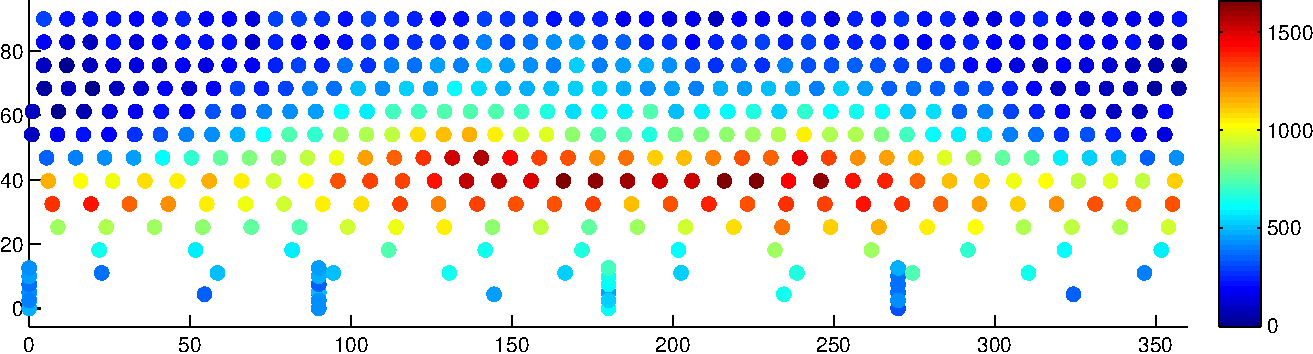
\includegraphics[width=10cm]{pic/scatter}}

\end{frame}


\subsection*{Exercises}

\begin{frame}
  
  \begin{block}{Exercises 1}
    \begin{enumerate}
      \item  Construct a vector \textbf{e} of all even numbers between 10 to 30.
      \item  Construct a vector \textbf{s} of the first 11 sqare numbers.
      \item  Set in \textbf{s} all values to 0 where \textbf{e} $>$ \textbf{s}!
    \end{enumerate}
  \end{block}

  \begin{block}{Exercises 2}
    \begin{enumerate}
    \item Load the file \texttt{data/juelich/104.hem} and plot the data as a
      scatter plot!
    \item Determin the minimum, maximum and mean
      intensity of the data!
    \item Plot a histogram of the intensities.
    \item Transform the data into cartesian coordinates and plot them!
    \item Remove all negative values from the data and plot them!
    \end{enumerate}
  \end{block}
\end{frame}



\section{Crystal Geometry}



\subsection*{Vector3d}

\begin{frame}[fragile]
  \frametitle{Specimen Directions - The \MTEX Class \texttt{\bf vector3d}}

  Definition: 

\begin{lstlisting}
v = vector3d(1,1,1);    % by Cartesian coordinate
v = sph2vec(theta,rho); % by polar coordinates
v = xvector;            % predefined vectors
\end{lstlisting}
  
  \medskip

  \begin{columns}
    \begin{column}{8.5cm}

      Calculations:
      
\begin{lstlisting}
v = [xvector,yvector]; w = v(1);              
v = 2*xvector-yvector; 
\end{lstlisting}
      
    \medskip
    
    Basic Functions:
    
\begin{lstlisting}
cross(v1,v2), dot(v1,v2)
norm(v), sum(v)
vec2sph(v)
\end{lstlisting}
  \end{column}
  \begin{column}{3cm}
   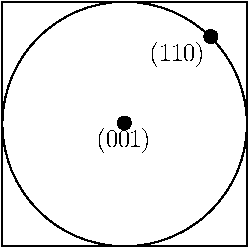
\includegraphics[width=3cm]{pic/vector3d}
  \end{column}
\end{columns}



\end{frame}

\subsection*{quaternion}


\begin{frame}[fragile]
  \frametitle{Rotations - The \MTEX Class \texttt{\bf quaternion}}

Definition:

\begin{lstlisting}
q = quaternion(a,b,c,d); 
q = axis2quat(axis,omega);  
q = euler2quat(alpha,beta,gamma); 
q = euler2quat(phi1,Phi,phi2,'Bunge'); 
q = Miller2quat([h k l],[u v w],CS); 
\end{lstlisting}
%q = idquaternion;         

\medskip

\begin{columns}
  \begin{column}{8.5cm}

    Calculations:
    
\begin{lstlisting}
q = [q1,q2]; q1 = q(1)
q = q1 * q2; w = q * v   
\end{lstlisting}
    
    \medskip
    
    Basic Functions:
    
\begin{lstlisting}
omega = rotangle(q)
v = rotaxis(q)
[alpha,beta,gamma]  = quat2euler(q)
\end{lstlisting}
    
  \end{column}
  
  \begin{column}{3cm}
    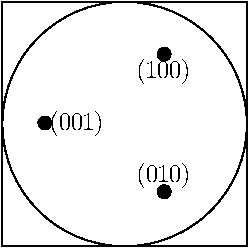
\includegraphics[width=3cm]{pic/quaternion}
  \end{column}

\end{columns}
\end{frame}

\subsection*{Symmetry} 
\begin{frame}[fragile]
  \frametitle{Crystal Symmetries - The \MTEX Class \texttt{\bf symmetry}}
  
  Definition:

\begin{lstlisting}
S = symmetry('triclinic',[a,b,c],[alpha,beta,gamma])
S = symmetry('-3m',[a,b,c]);
S = symmetry('O'); 
\end{lstlisting}

\medskip

\begin{columns}
  \begin{column}{8.5cm}

Load Symmetry from CIF file:

\begin{lstlisting}
cif2symmetry('quartz.cif')
\end{lstlisting}

\medskip

    Basic Functions:

\begin{lstlisting}
symmetriceVec(SS,v)
dist(CS,SS,q1,q2)   
quaternion(CS)
getFundamentalRegion(CS)
\end{lstlisting}
  \end{column}
  
  \begin{column}{3cm}
    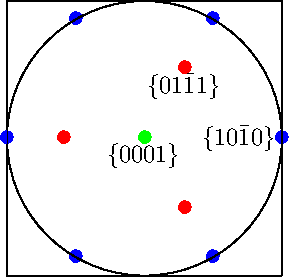
\includegraphics[width=3cm]{pic/sym}
  \end{column}

\end{columns}

\end{frame}

\subsection*{Miller}

\begin{frame}[fragile]
  \frametitle{Crystal Directions - The \MTEX Class \texttt{\bf Miller}}
  
  Definition:

\begin{lstlisting}
h = Miller(1,0,0,CS);
h = [Miller(1,1,-2,3,CS),Miller(0,1,-1,0,CS)]
h = vec2Miller(v,CS);
\end{lstlisting}

\medskip

\begin{columns}
  \begin{column}{8.5cm}

    Calculations:

\begin{lstlisting}
q * Miller(1,0,0,CS)
q * symeq(Miller(1,0,0,CS))
\end{lstlisting}

\medskip

    Basic Functions:

\begin{lstlisting}
symeq(h1,h2)
symvec(h)
angle(h1,h2)
\end{lstlisting}
  \end{column}
  
  \begin{column}{3cm}
    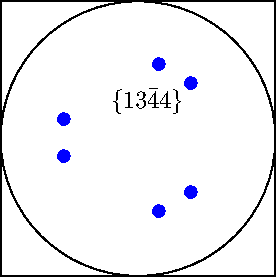
\includegraphics[width=3cm]{pic/miller}
  \end{column}

\end{columns}

\end{frame}

\subsection*{S2Grid}


\begin{frame}[fragile]
  \frametitle{Sets of Specimen Directions - The \MTEX Class \texttt{\bf S2Grid}}
  
Definition:

\begin{lstlisting}
S2G = S2Grid('regular','resolution',5*degree);
S2G = S2Grid('regular','maxrho',80*degree);
S2G = S2Grid('equispaced','points',10000);     
\end{lstlisting}

\medskip

Basic Functions:

\begin{lstlisting}
add, delete, rotate, union, subGrid, refine,
GridLength, getResolution, getRho, getTheta, 
polar, vector3d
\end{lstlisting}

\onslide<1->
\begin{center}
  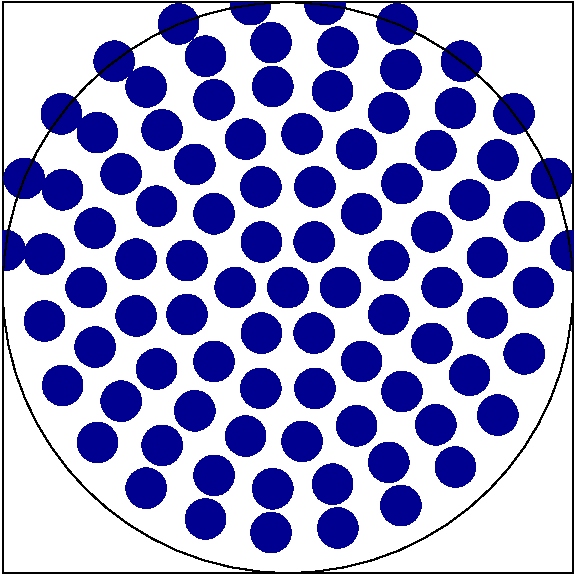
\includegraphics[width=2.5cm]{pic/S2Grid1} \quad
  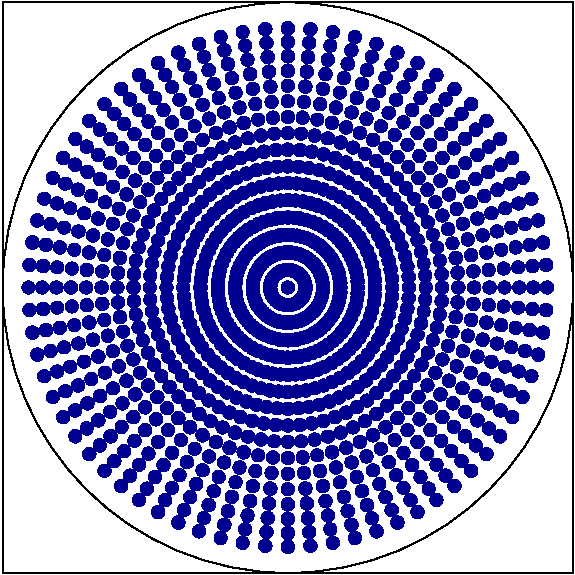
\includegraphics[width=2.5cm]{pic/S2Grid2} \quad
  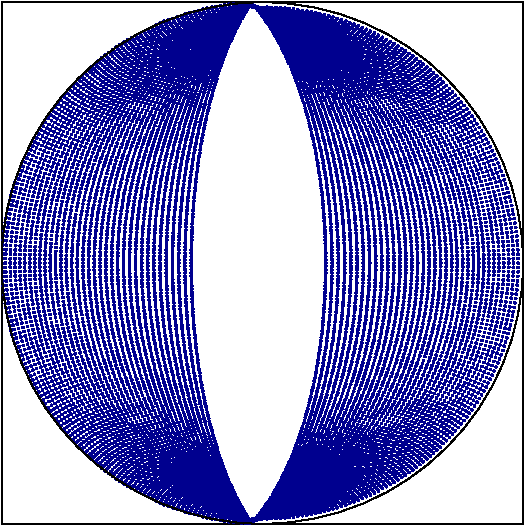
\includegraphics[width=2.5cm]{pic/S2Grid3} \quad
  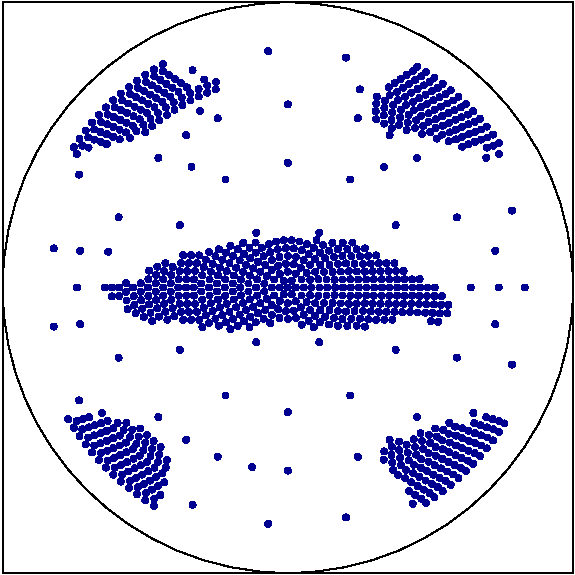
\includegraphics[width=2.5cm]{pic/S2Grid4}
\end{center}

\end{frame}


\subsection*{Exercises}

\begin{frame}
  
  \begin{block}{Exercise 3}
 Consider trigonal crystal symmetry.

 \begin{enumerate}
 \item Find all crystallographic directions symmetrically equivalent to (1, 0,
   − 1, 0) (Miller indices)!
 \item Find crystallographic directions such that the number of their
   crystallographic equivalent directions on the upper hemisphere (without
   equator) is 1, 3, or 6?
 \item Construct an orientation that rotates the crystallographic directions
   $(1,0,0)$ and $(0,1,0)$ onto $(0,0,0,1)$ and $(2,-1,-1,0)$, respectively.
 \item Find all crystallographic equivalent orientations to
   $(45\degree,0\degree,0\degree)$ (Euler angle) and give its Euler angles!
 \item Find all crystallographic equivalent specimen directions to the crystal
   direction $(1,1,-2,1)$ under the orientation
   $(45\degree,0\degree,0\degree)$ (Euler angle)!
 \end{enumerate}

\end{block}




\end{frame}

\section{Model ODFs}


\subsection*{ODFs in MTEX}


\begin{frame}[fragile]
  \frametitle{Orientation Density Functions in \MTEX}


  \centering{
    \includegraphics[width=10cm]{latex_pic/odf}
  }

\end{frame}

\subsection*{ODFs in MTEX}


\subsection*{The Class kernel}


\begin{frame}[fragile]
  \frametitle{The Shape of the ODF -- The \MTEX Class \texttt{\bf kernel}}

Definition:

\begin{lstlisting}
psi = kernel('de la Vallee Poussin',80);
psi = kernel('Abel Poisson','halfwidth',10*degree);
\end{lstlisting}

\medskip

Supported kernel functions:

\begin{quote}
  Abel -- Poisson, de la Vall\'ee Poussin, von Mises -- Fisher, fibre von Mises
  -- Fisher, Gauss -- Weierstrass, Dirichlet, Bump
\end{quote}

Plot of the \textcolor{blue}{Abel Poisson}, the \textcolor{red}{Dirichlet} and
the \textcolor{green}{Bump} kernel:

\onslide<1->
\begin{center}
  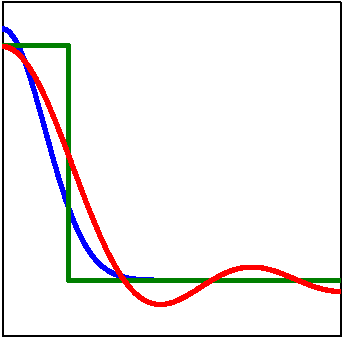
\includegraphics[width=3.5cm]{pic/K} \quad
  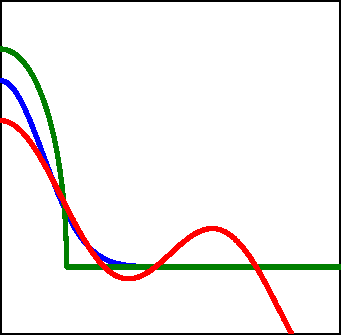
\includegraphics[width=3.5cm]{pic/RK} \quad
  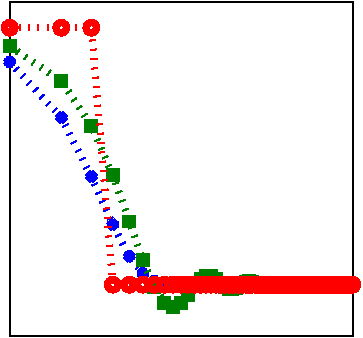
\includegraphics[width=3.5cm]{pic/Fourier}
\end{center}
  
\end{frame}

\subsection*{Unimodal ODFs}

\begin{frame}[fragile]
  \frametitle{Defining Unimodal ODFs in \MTEX}

\begin{columns}   
    
  \begin{column}{8.5cm}
    
      Characteristics of an unimodal ODF:
      \begin{enumerate}
      \item crystal symmetry
      \item specimen symmetry
      \item modal orientation
      \item kernel function
      \end{enumerate}

  

\begin{lstlisting}
SS = symmetry('orthorhombic')
CS = symmetry('cubic')
q = Miller2quat([1 2 2],[2 2 1],CS);
psi = kernel('von Mises Fisher',...
             'halfwidth',20*degree);
\end{lstlisting}

      \begin{actionenv}<1-| alert@1->
\begin{lstlisting}
odf = unimodalODF(q,CS,SS,psi)
\end{lstlisting}
    \end{actionenv}

\end{column}
    
    \begin{column}{3cm}
      \onslide<1->  
      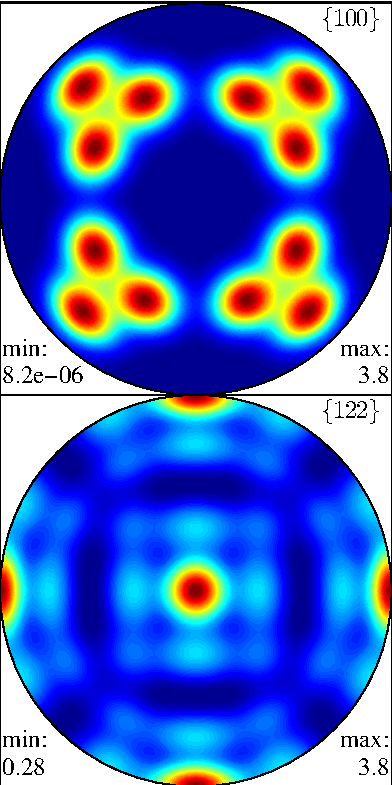
\includegraphics[width=3cm]{pic/unimodalODF}
    \end{column}
  \end{columns}
  
\end{frame}



\subsection*{Fibre ODFs}

\begin{frame}[fragile]
  \frametitle{Defining Fibre ODFs in \MTEX}

  \begin{columns}   
  
    \begin{column}{8.5cm}
    
      Characteristics of an Fibre ODFs:
      \begin{enumerate}
      \item crystal symmetry
      \item specimen symmetry
      \item crystal direction
      \item specimen direction
      \item kernel function
      \end{enumerate}
 

\begin{lstlisting}
SS = symmetry('triclinic')
CS = symmetry('hexagonal')
h = Miller(1,0,0,CS);
r = xvector;
psi = kernel('Abel Poisson',...
             'halfwidth',18*degree);
\end{lstlisting}

      \begin{actionenv}<1-| alert@1->
\begin{lstlisting}
odf = fibreODF(h,r,CS,SS,psi)
\end{lstlisting}
      \end{actionenv}

\end{column}
    
    \begin{column}{3cm}
      \onslide<1->  
      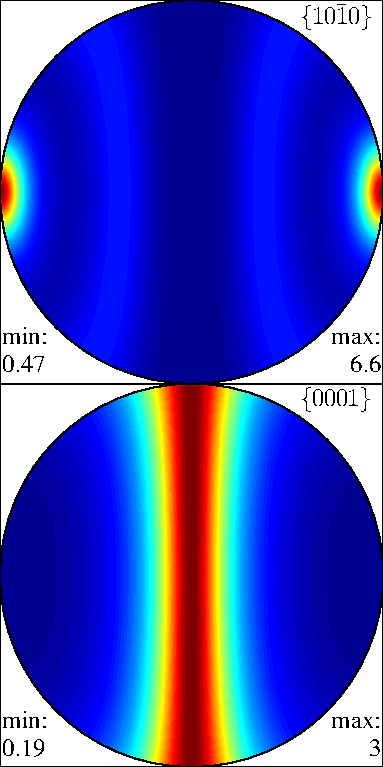
\includegraphics[width=3cm]{pic/fibreODF}
    \end{column}
  \end{columns}


\end{frame}

\subsection*{Fourier ODFs}

\begin{frame}[fragile]
  \frametitle{Defining Uniform and  Fourier ODFs}

  The uniform ODF:
\begin{lstlisting}
SS = symmetry('triclinic')
CS = symmetry('hexagonal')
\end{lstlisting}

  \begin{actionenv}<1-| alert@1->
\begin{lstlisting}
 odf = uniformODF(CS,SS)
\end{lstlisting}
  \end{actionenv}  

  \begin{block}{Fourier expansion of an ODF}
    \begin{equation*}
      f(\vec g) = \sum_{l=0}^L \sum_{k,k'=-l}^l C_l^{k,k'} T_l^{k,k'}(\vec g)
    \end{equation*}
    \begin{equation*}
      C = [C_0,C_1^{-1,-1},C_1^{0,-1},C_1^{1,-1},\ldots,C_1^{1,1},C_2^{-2,-2},\ldots,C_L^{L,L}]
    \end{equation*}
  \end{block}
The Fourier ODF:
  \begin{actionenv}<1-| alert@1->
\begin{lstlisting}
odf = FourierODF(C,CS,SS)
\end{lstlisting}
  \end{actionenv}  



\end{frame}

\subsection{ODF Arithmetic}

\begin{frame}[fragile]
  \frametitle{ODF Arithmetic}


  \begin{columns}
    \begin{column}{6cm}
        
      Calculate with ODFs:
\begin{lstlisting}
odf1 = unimodalODF(...)
odf2 = fibreODF(...)
odf3 = uniformODF(CS,SS)

odf = 0.2*odf1 + 0.3*odf2 
      + 0.5*odf3 

\end{lstlisting}
  
  Rotate ODFs:
\begin{lstlisting}
q = axis2quat(xvector,...
              90*degree);
odf = rotate(odf,q)       
\end{lstlisting}


  Standard ODFs:
\begin{lstlisting}
odf = santafee; 
\end{lstlisting}

        
\end{column}
\begin{column}{5cm}
  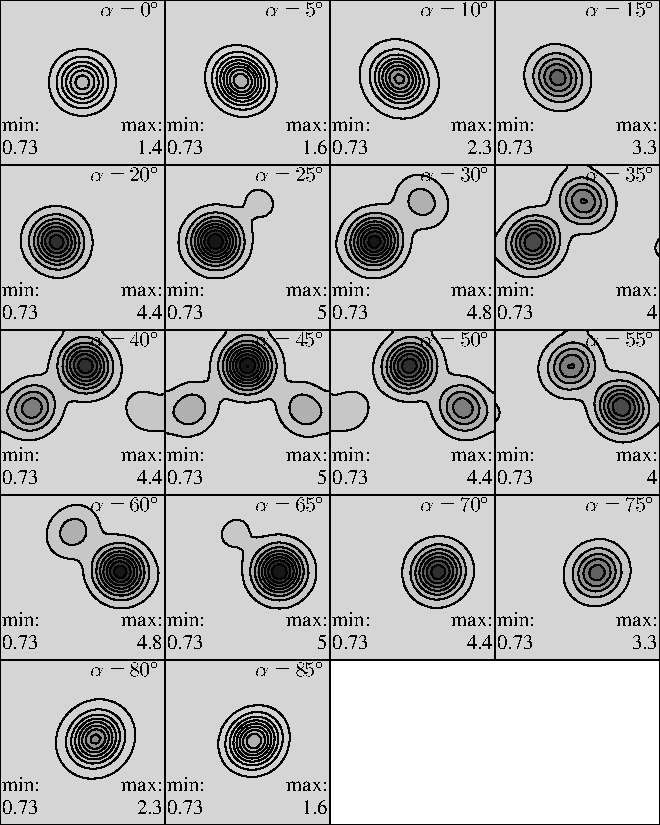
\includegraphics[width=5cm]{pic/santafeeh}
\end{column}
\end{columns}    

\end{frame}

\section*{ODF Analysis}

\subsection*{Working with ODFs}

\begin{frame}
  \frametitle{Analyzing and Visualizing ODFs in \MTEX}

  \begin{center}
    \includegraphics[width=10cm]{latex_pic/odf2}
  \end{center}
\end{frame}

\subsection*{Working with ODFs}

\begin{frame}[fragile]
  \frametitle{Texture Characteristics}

Comparing {\bf arbitrary} ODFs
\begin{lstlisting}
calcerror(odf1,odf2,'L1')
\end{lstlisting}

\pause

Volume portions: 
\begin{lstlisting}
volume(odf,center,radius) % the volume within a ball
fibrevolume(odf,h,r,radius) % the volume of a fibre
\end{lstlisting}

\pause

Preferred orientations:
\begin{lstlisting}
q = modalorientation(odf) % the modal orientation
q = mean(odf)             % the mean orientation 
\end{lstlisting}

\pause

The shape of the ODF:
\begin{lstlisting}
textureindex(odf)         % the texture index
entropy(odf)              % the entropy
fourier(odf,order)        % the C-coefficients     
\end{lstlisting}


\end{frame}


\subsection*{Plotting (Inverse) Pole Figures}

\begin{frame}[fragile]
  \frametitle{Plotting (Inverse) Pole Figures in \MTEX}
  
  General syntax:
\begin{lstlisting}
plotpdf(odf,Miller(0,1,0),<options>)
plotipdf(odf,[xvector,zvector],<options>)
\end{lstlisting}

Options:
\begin{lstlisting}
reduced  % plot only northern hemisphere
complete % plot complete hemisphere
\end{lstlisting}


\onslide<1->
\center{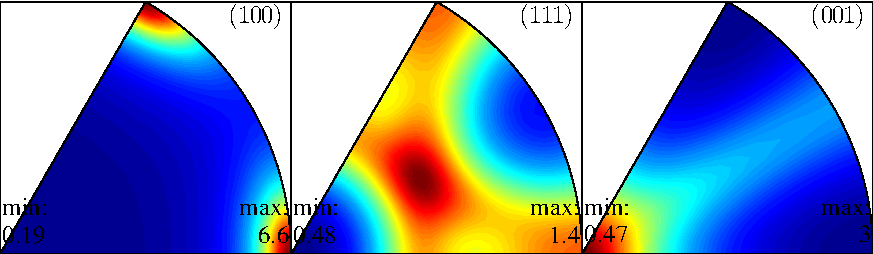
\includegraphics[height=3cm]{pic/ipdf}}

\end{frame}


\subsection*{Plotting an ODF}

\begin{frame}[fragile]
  \frametitle{Plotting  an ODF in \MTEX}

  \begin{columns}
    \begin{column}{6.5cm}
      General syntax:
\begin{lstlisting}
plot(odf,<options>)
\end{lstlisting}
      
      Sectioning:
      \lstset{emph={sigma},emphstyle={\color{blue}}}
\begin{lstlisting}
alpha, gamma, phi1, phi2
sigma, radially
\end{lstlisting}
      
      Options:
\begin{lstlisting}
sections, center, axes
\end{lstlisting}

      Example:      
    \end{column}
    \begin{column}{5cm}
      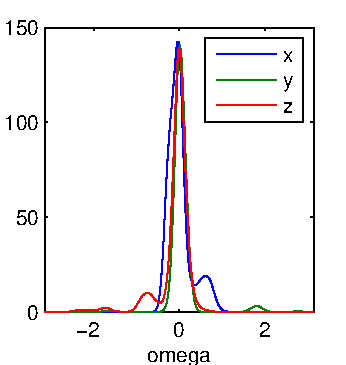
\includegraphics[width=5cm]{pic/radialplot}
    \end{column}
  \end{columns}

\begin{lstlisting}
plot(odf,'radially',...
  'center',modalorientation(odf),...
  'axes',[xvector,yvector,zvector])
\end{lstlisting}

%\begin{lstlisting}
%plot(odf,'alpha',[45*degree])
%\end{lstlisting}

\end{frame}


\subsection*{Dubna}

\begin{frame}[fragile]
  \frametitle{A Sigma Plot of the Recalculated Dubna ODF in \MTEX}

\begin{lstlisting}
plot(rec,'sections',18,'FontSize',10)
\end{lstlisting}

\medskip

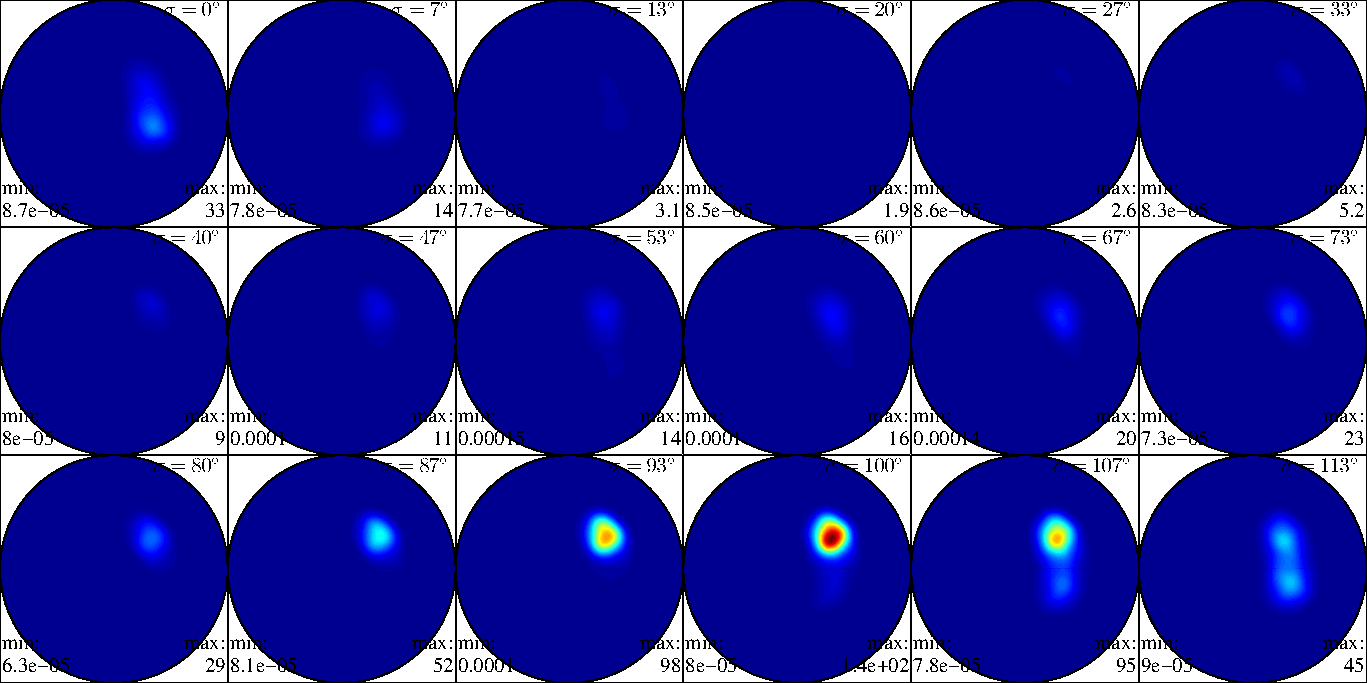
\includegraphics[width=\textwidth]{pic/ODFso9}
  
\end{frame}

\subsection*{Santafee}

\begin{frame}[fragile]
  \frametitle{The Classical Plot of the Santafee ODF in \MTEX}

\begin{lstlisting}
plot(santafee,'alpha','sections',18,...
     'projection','plain','gray','contourf')
\end{lstlisting}

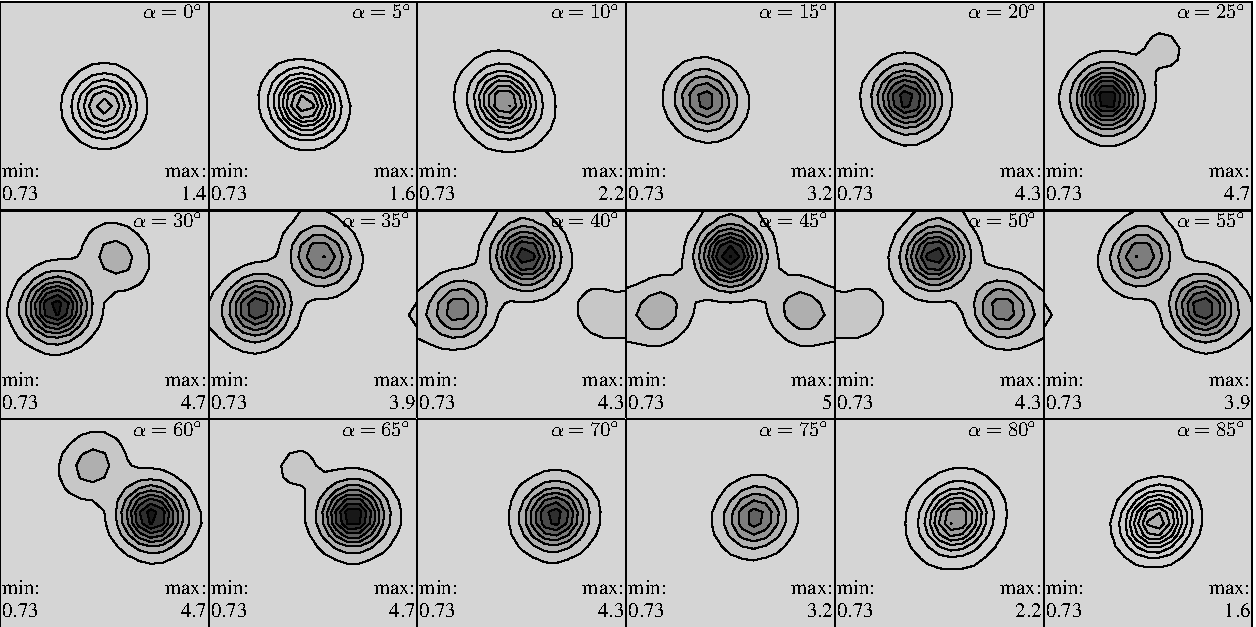
\includegraphics[width=\textwidth]{pic/santafee}
  
\end{frame}


\section{Pole Figures}

\subsection*{Layout}

\begin{frame}[fragile]
  \frametitle{Experimental Pole Figures in \MTEX}

  \begin{columns}

    \begin{column}{8.2cm}

      Characteristics of a single experimental pole figure in \mtex:
      \begin{enumerate}
      \item vector of superposed crystal directions
      \item vector of structure coefficients
      \item set of specimen directions
      \item vector of diffraction intensities
      \item crystal symmetry
      \item specimen symmetry
      \item background radiation intensities (optional)
      \end{enumerate}

    \end{column}

    \begin{column}{3cm}
      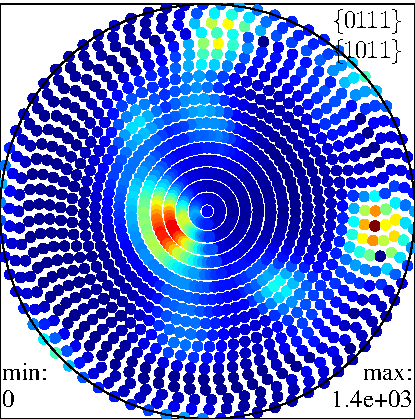
\includegraphics[width=3cm]{pic/pf1}\\
      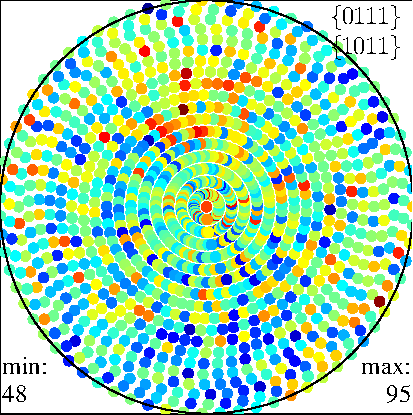
\includegraphics[width=3cm]{pic/pfso9_bg}
    \end{column}


  \end{columns}


\end{frame}


\subsection*{Construction (low level)}



\begin{frame}[fragile]
  \frametitle{Importing Pole Figure Data - The Import Wizard}

  \begin{columns}

    \begin{column}{6cm}
      Formats supported by \MTEX:
      \begin{itemize}
      \item Popla: *.EPF
      \item BearTex: *.XPa
      \item Dubna: *.cnv, *.cns
      \item Geesthacht
      \item Aachen: *.exp
      \item Philips: *.txt
      \item J\"ulich: *.hem
      \item *.nja
      \item *.ptx
      \item *.plf
      \item *.xrdml
      \item generic ascii files
      \end{itemize}


    \end{column}
    
    \onslide<1->

    \begin{column}{6cm}
      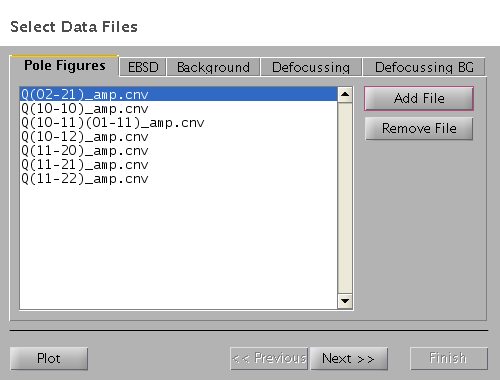
\includegraphics[width=6cm]{pic/iw}
    \end{column}

  \end{columns}

\end{frame}

\subsection*{Construction (high level)}

\begin{frame}[fragile]
  \frametitle{Importing Pole Figure Data Using a Script}

  \begin{columns}
    \begin{column}{8.5cm}
      
\begin{lstlisting}
CS = symmetry('-3m',[1.2 1.2 3.5]);
SS = symmetry('triclinic');
\end{lstlisting}
  
\pause

\begin{lstlisting}
pf_files = {'Q(10-10).cnv',...
            'Q(10-11)(01-11).cnv',...
            'Q(11-22).cnv'};

h = {Miller(1,0,-1,0,CS),...
     [Miller(0,1,-1,1,CS),...
      Miller(1,0,-1,1,CS)],...
     Miller(1,1,-2,2,CS)};

c = {1,[0.52,1.23],1};
\end{lstlisting}        
      
\pause

      \begin{actionenv}<1-| alert@1->  
\begin{lstlisting}
pf = loadPoleFigure(pf_files,h,...
       CS,SS,'superposition',c);
\end{lstlisting}
      \end{actionenv}
  
    \end{column}

    \begin{column}{3cm}
      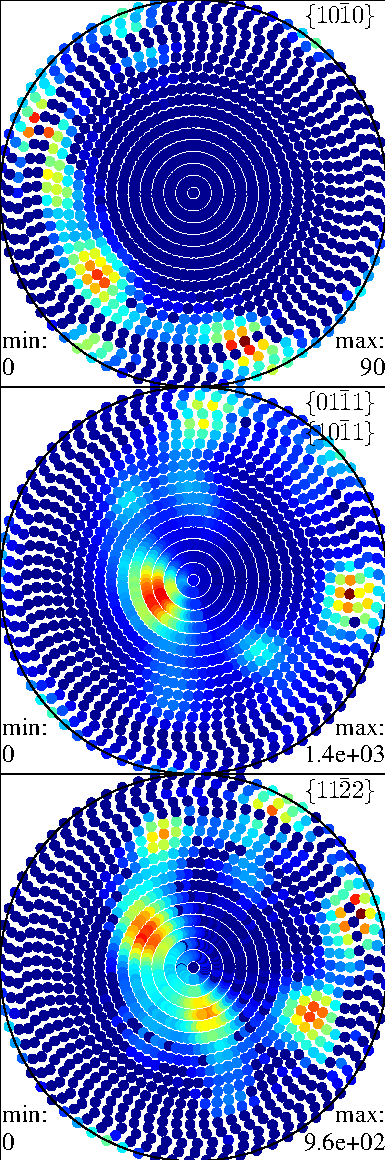
\includegraphics[width=2.5cm]{pic/pforig}
    \end{column}
    
  \end{columns}
  
\end{frame}


\subsection*{Analyze Diffraction Data}

\begin{frame}[fragile]
  \frametitle{Using \MTEX to Analyze Diffraction Data}



Retrieve information from pole figures:
\begin{lstlisting}
I = get(pf,'data')   % the intensities
h = get(pf,'Miller') % the Miller indice
r = get(pf,'r')      % the specimen directions
\end{lstlisting}

Basic Statistics:
\begin{lstlisting}
min(pf), max(pf), hist(pf), find_outlier(pf)
\end{lstlisting}

\center{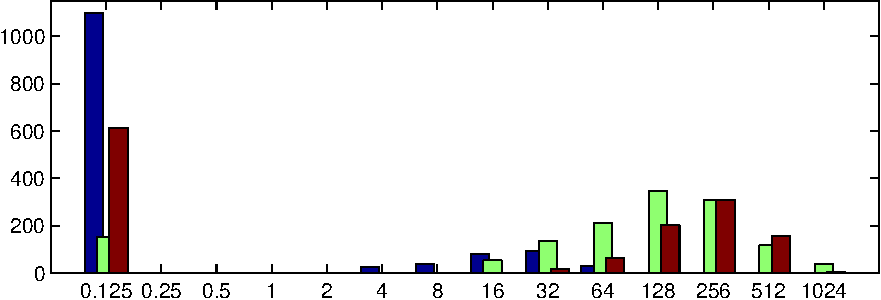
\includegraphics[height=3cm]{pic/hist}}

\end{frame}

\subsection*{Modify Pole Figures}

\begin{frame}[fragile]

  \frametitle{Using \MTEX to Modify Pole Figures}

  \begin{columns}
  
    \begin{column}{8.5cm}

      Pole figure arithmetics:
\begin{lstlisting}
pf = 2*pf1 + 5*pf2;
pf = [pf1,pf2]; 
pf = pf([1,3,5]);
\end{lstlisting}
      
      Pole figure modification:
      
\begin{lstlisting}
scale(pf,alpha),
union(pf1,pf2), 
delete(pf,indices), 
rotate(pf,q),
setdata(pf,value,indices)
\end{lstlisting}
      
      \begin{overprint}

        \onslide<2|handout:1>
        Example:
\begin{lstlisting}
theta = get(pf,'polar');
pf = delete(pf,theta >= 70*degree ...
   & theta <= 75*degree)
\end{lstlisting}
        \onslide<3|handout:0>
        Example:
\begin{lstlisting}
pf = rotate(pf,axis2quat(...
      xvector-yvector,25*degree))

\end{lstlisting}
        \onslide<4|handout:0>
        Example:
\begin{lstlisting}
pf = setdata(pf,1,get(pf,'data')<1)
\end{lstlisting}
        
      \end{overprint}
    \end{column}

    \begin{column}{3.1cm}
      \onslide<1->
      \only<1|handout:0>{%
        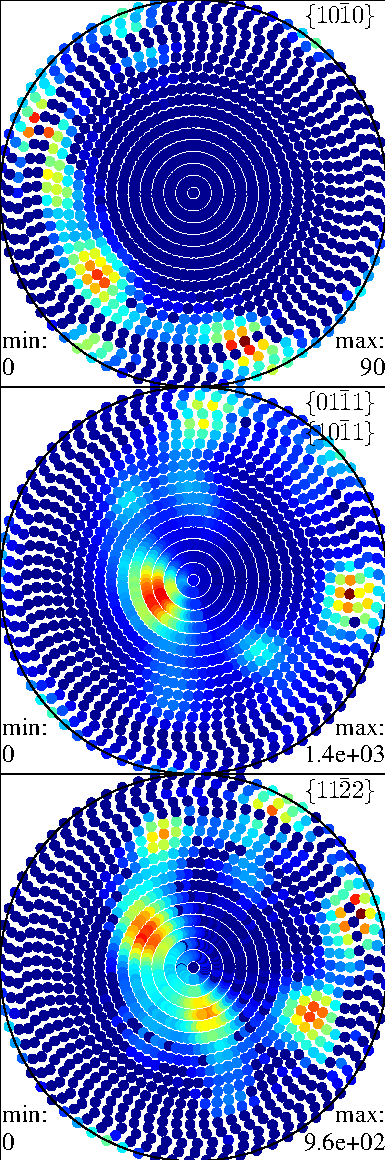
\includegraphics[height=7.5cm]{pic/pforig}%
      }%
      \only<2>{%
        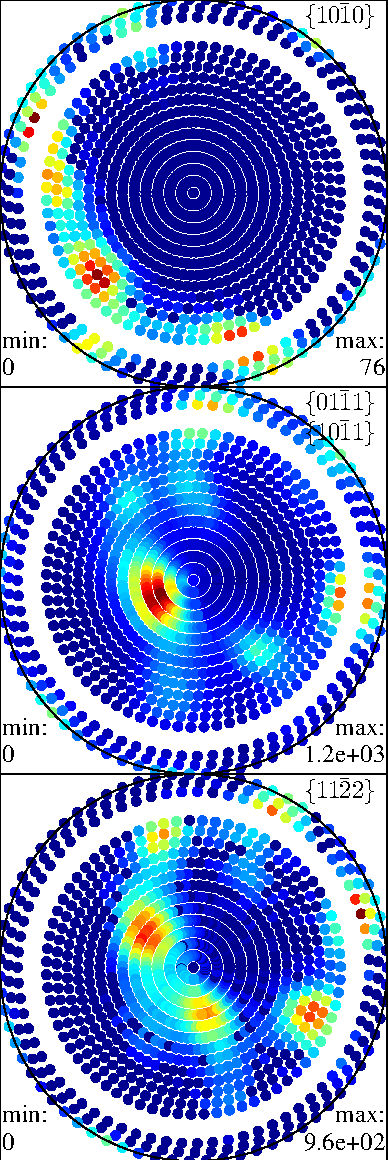
\includegraphics[height=7.5cm]{pic/pfdelted}%
      }%
      \only<3|handout:0>{%
        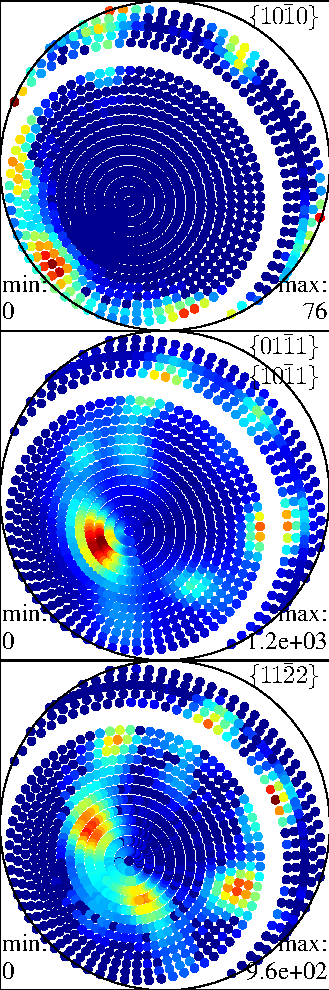
\includegraphics[height=7.5cm]{pic/pfrotated}%
      }%
      \only<4|handout:0>{%
        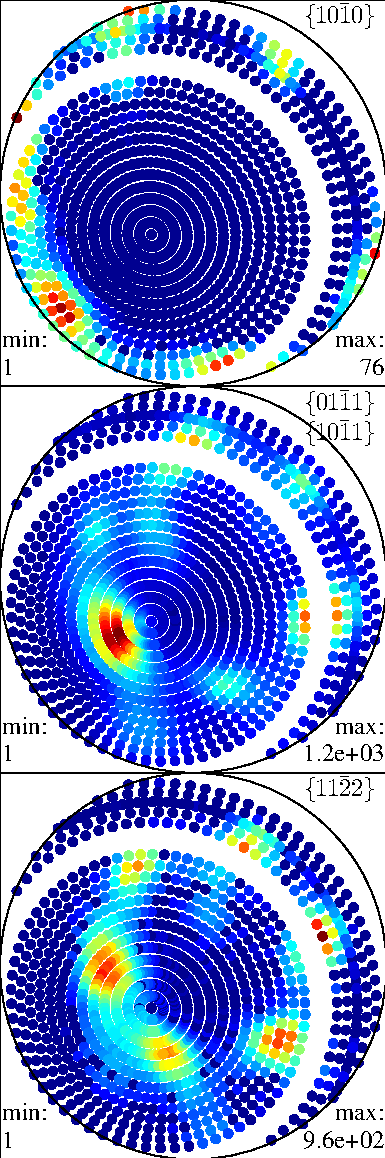
\includegraphics[height=7.5cm]{pic/pfincreased}%
      }
    \end{column}

  \end{columns}

\end{frame}

\subsection*{PDF - to - ODF Reconstruction}


\begin{frame}[fragile]
  \frametitle{PDF to ODF Reconstruction in \MTEX}

  Syntax:
  \begin{alertenv}
\begin{lstlisting}
odf = calcODF(pf,<options>)
\end{lstlisting}
  \end{alertenv}

Options:
\lstset{emph={bandwidth},emphstyle={}}
\begin{lstlisting}
resolution, kernelwidth, bandwidth
iter_min, iter_max
zero_range       
ghost_correction 
\end{lstlisting}

\pause

\begin{table}[H]
  \centering
  \begin{tabular}{r r r r}
    \toprule
    resolution & kernelwidth  & bandwidth & time \\
    \midrule
    $20^\circ$  & $26.7^\circ$ & 23  & 3s   \\
    $10^\circ$  & $13.3^\circ$ & 52  & 28s  \\
    $5^\circ$   & $6.7^\circ$  & 108 & 3min \\
    $2.5^\circ$ & $3.3^\circ$  & 215 & 30min\\
    $1.5^\circ$ & $2^\circ$    & 300 & 1.5h\\
    \bottomrule
  \end{tabular}  
\end{table}

\end{frame}


\subsection*{Santafee}

\begin{frame}[fragile]
  \frametitle{ODF Reconstruction Without Ghost Correction}

\begin{lstlisting}
rec = calcODF(pf_santafee,'RESOLUTION',10*degree,...
              'background',1,'iter_max',6)
\end{lstlisting}

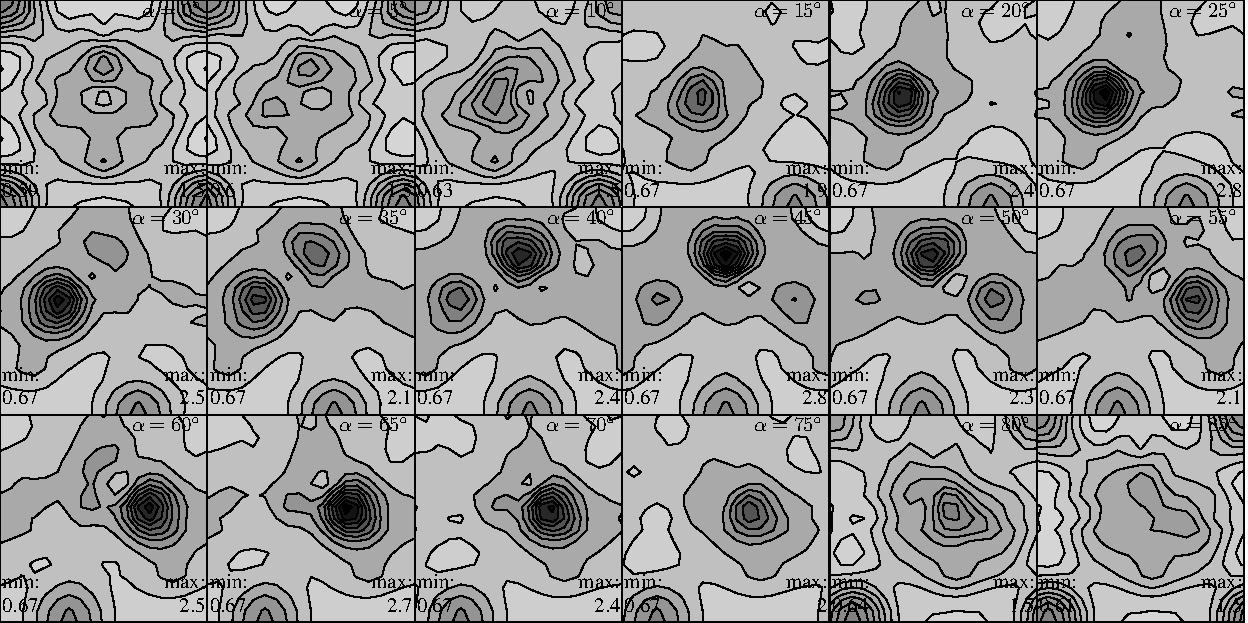
\includegraphics[width=\textwidth]{pic/rec_santafee}
  
\end{frame}
\subsection*{Santafee}

\begin{frame}[fragile]
  \frametitle{ODF Reconstruction With Ghost Correction}

\begin{lstlisting}
rec = calcODF(pf_santafee,'RESOLUTION',10*degree,...
 'background',10,'iter_max',6,'ghost_correction')
\end{lstlisting}

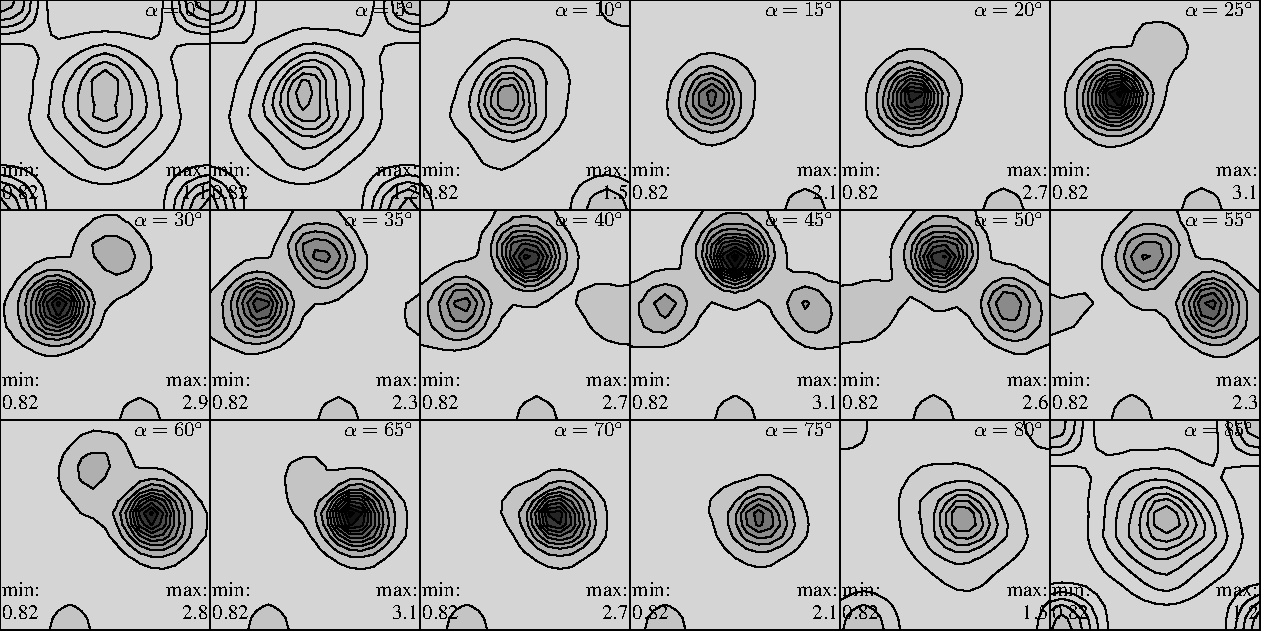
\includegraphics[width=\textwidth]{pic/rec_santafee_ghost_correction}
  
\end{frame}


\subsection*{Error Analysis}

\begin{frame}[fragile] 
  \frametitle{Error Analysis of Reconstructed ODFs in  \MTEX}
  
Estimate reconstruction error:
\begin{lstlisting}
e = calcerror(pf,odf,<options>)
\end{lstlisting}

Options:
\begin{lstlisting}
RP, L1, L2
\end{lstlisting}

Difference plot:
\begin{lstlisting}
plotDiff(pf,odf,<options>)
\end{lstlisting}

\center{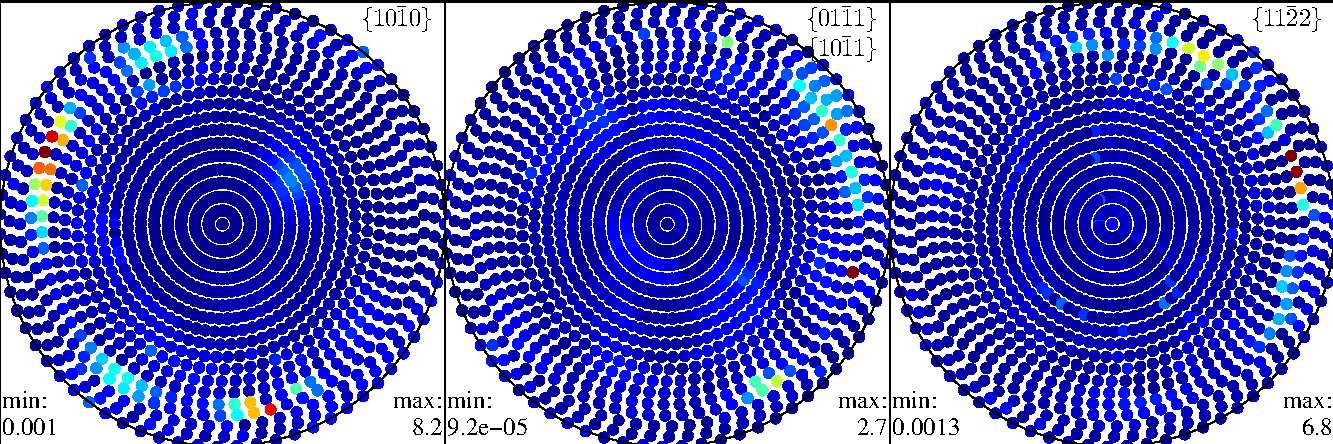
\includegraphics[height=3cm]{pic/diffpf}}

\vspace{3mm}

\end{frame}

\subsection{Pole Figure Simulation}

\begin{frame}[fragile]
  \frametitle{Pole Figure Simulation in \mtex}

  \begin{columns}
    \begin{column}{8cm}

      Simulation of pole figure data may help to analyze the error made by ODF
      reconstruction from real data.

\begin{lstlisting}
%define a model ODF
odf = santafee                  

% define crystal directions
h = [Miller(1,0,0], Miller(1,1,0)]

% define specimen directions
r = S2Grid('regular','reduced') 

% simulate pole figure data
pf = simulatePoleFigure(odf,h,r)
\end{lstlisting}      
    \end{column}

    \begin{column}{4cm}
      \centerline{
      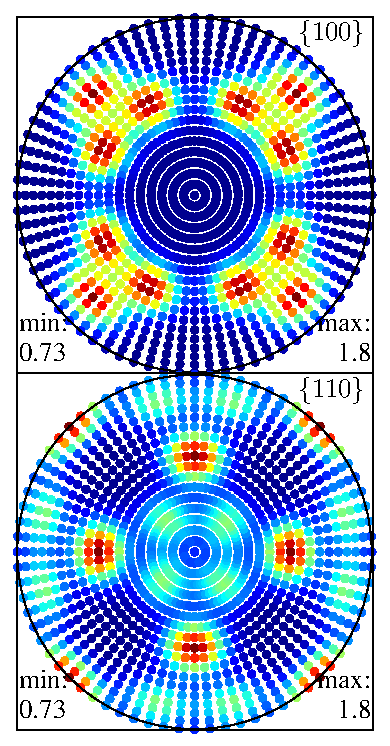
\includegraphics[width=4cm]{pic/simpf}}
    \end{column}

  \end{columns}
 
\end{frame}

\subsection{Reconstruction Error}

\begin{frame}
  \frametitle{Reconstruction Error vs. Number of Pole Figures}

  \center{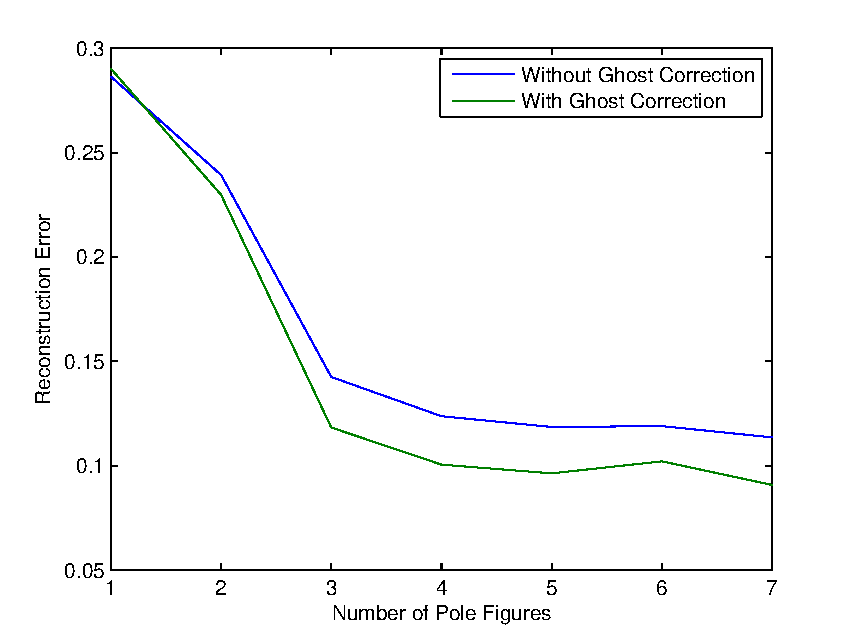
\includegraphics[width=10cm]{pic/pfcorrectness}}
  
\end{frame}




\section{EBSD}

\subsection*{EBSD}


\begin{frame}[fragile]
  \frametitle{Single Orientation Meassurments}

  \begin{columns}

    \begin{column}{7.2cm}

      Characteristics of a EBSD data in \mtex:
      \begin{enumerate}
      \item vector of orientations
      \item crystal symmetry
      \item specimen symmetry
      \item spatial coordinates
      \item phase information
      \item data reliability
      \end{enumerate}

\begin{lstlisting}
CS = symmetry('cubic')
SS = symmetry('triclinic')
ebsd = loadEBSD(fname,CS,SS,...
  'layout',[5 6 7],'xy',[3 4]);

plot(ebsd)
\end{lstlisting}

    \end{column}

    \begin{column}{4cm}
      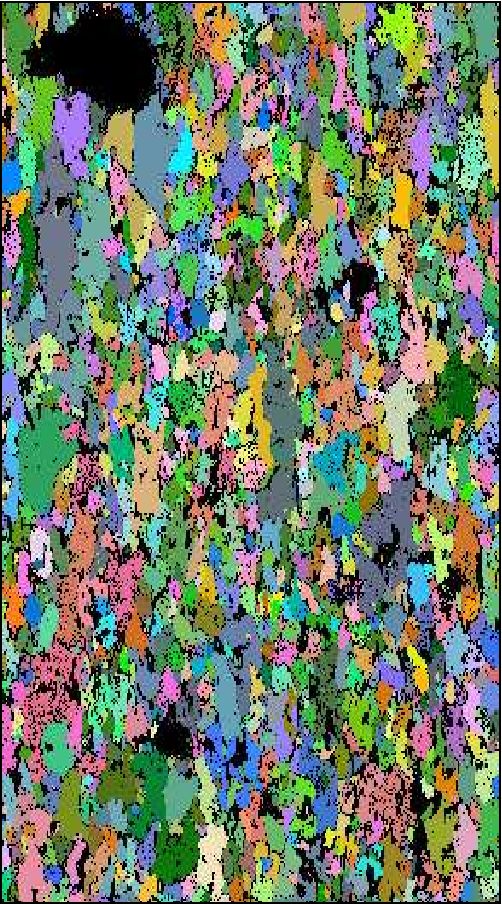
\includegraphics[width=4cm]{pic/ebsd}
    \end{column}


  \end{columns}
  
\end{frame}

\subsection{Working With EBSD Data}

\begin{frame}[fragile]
  \frametitle{Working With EBSD Data}
  
  \begin{columns}
    \begin{column}{8.5cm}
Extracting Data
\begin{lstlisting}
orientations = get(ebsd,'data')
x = get(ebsd,'x')
\end{lstlisting}

\medskip

Modify EBSD Data
\begin{lstlisting}
rot = axis2quat(xvector,90*degree)
ebsd = rotate(ebsd,rot) 
ebsd = [ebsd_1,ebsd_2] 
ebsd = delete(ebsd,x > 100)
\end{lstlisting}

\medskip

Plot Pole Figures of EBSD Data
\begin{lstlisting}
plotpdf(ebsd,[Miller(0,0,0,1),...
  Miller(1,0,-1,0)])
\end{lstlisting}      
    \end{column}

    \begin{column}{3.5cm}
      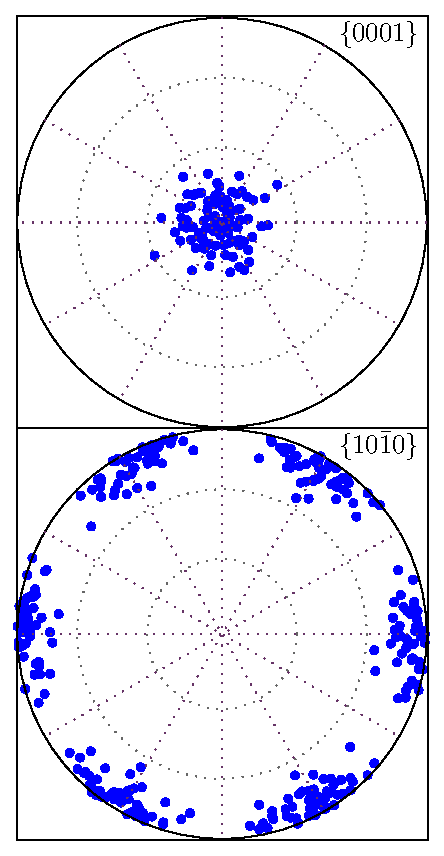
\includegraphics[width=3.5cm]{pic/EBSDpdf}
    \end{column}
  \end{columns}



\end{frame}


\subsection*{EBSD - to - ODF Reconstruction}


\begin{frame}[fragile]
  \frametitle{EBSD to ODF Reconstruction in \MTEX}

  \mtex uses kernel density estimation to define an ODF from given single
  orientation measurements. The sensitive parameter of this method is the
  kernel function.

\medskip

  Syntax:
  \begin{alertenv}
\begin{lstlisting}
odf = calcODF(pf,<options>)
\end{lstlisting}
  \end{alertenv}

Options:
\lstset{emph={bandwidth},emphstyle={}}
\begin{lstlisting}
'kernel'     % the kernel to be used 
'halfwidth'  % halfwidth of the kernel function
'resolution' % resolution of the approximation grid
\end{lstlisting}


\end{frame}

\subsection{EBSD Simulation}

\begin{frame}[fragile]
  \frametitle{EBSD Simulation in \mtex}

  Simulation of EBSD data may help to analyze the error made by ODF kernel
  density estimation from real data.

\begin{lstlisting}
ebsd = simulateEBSD(santafee,5000) 
\end{lstlisting}      

Compute the error between the original ODF and the estimated ODF.
\begin{lstlisting}
error = calcerror(santafee,calcODF(ebsd))
\end{lstlisting}      

      \centerline{
      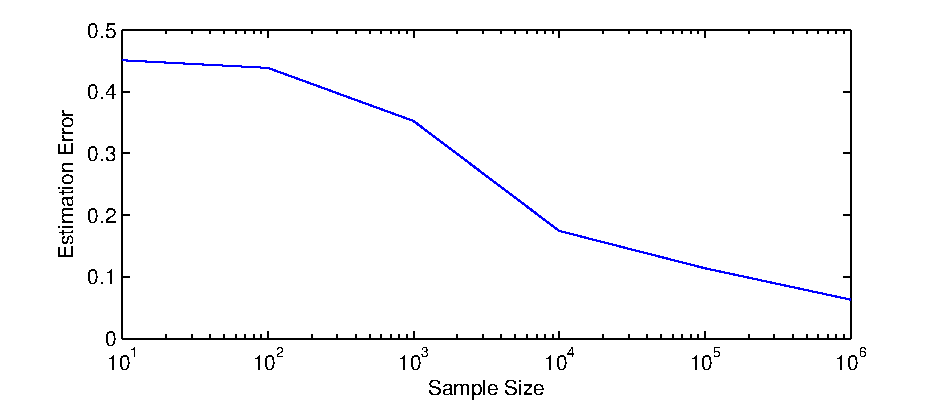
\includegraphics[width=10cm]{pic/ebsdcorrectness}}
 
\end{frame}


\subsection*{Exercises}

\begin{frame}
  
  \begin{block}{Exercises 4}
    \begin{enumerate}
    \item Load the EBSD data set
      \texttt{data/ebsd\_txt/85\_829grad\_07\_09\_06.txt} and estimate an ODF!
    \item Plot the ODF and some of its pole figures!
    \item Explore the influence of the halfwidth to the kernel 
      density estimation by looking at the pole figures!
    \end{enumerate}
  \end{block}
  
  \begin{block}{Exercises 5}
    \begin{enumerate}
    \item Start with an arbitrary model ODF!
    \item Compute the volume portion of the ODF within a range of $20\degree$
      of the modalorientation and compare it to the corresponding volume of
      the uniform ODF!
    \item Simulate EBSD data from this ODF with 10.000 orientations.
    \item Plot pole figures from the EBSD data and compare them with the pole
      figures from the model ODF.
    \item Compute the volume portion of the estimated ODF within a range of
      $20\degree$ of the modalorientation and compare it to model ODF!
    \item Perform these investigations for different sample sizes!
    \end{enumerate}
  \end{block}

\end{frame}



\section{Plotting}


\subsection*{Basic Plotting Tools}

\begin{frame}[fragile]
  \frametitle{Basic \MTEX Plotting Tools}

General syntax:
\begin{lstlisting}
plot(object,<options>)
\end{lstlisting}

\begin{columns}
  \begin{column}{8.5cm}

    \only<1>{
      \lstset{emph={tight,jet,earea,smooth,reduced},emphstyle={\color{blue}}}
    }
    
    \only<2|handout:0>{
      \lstset{emph={tight,jet,edist,smooth,reduced},emphstyle={\color{blue}}}     
    }
    
    \only<3|handout:0>{
      \lstset{emph={equal,earea,contourf,gray,reduced},emphstyle={\color{blue}}}
    }
    
    
    Color range:
  
\begin{lstlisting}
tight, equal, [min max]
\end{lstlisting}       
 
    Spherical projections:
\begin{lstlisting}
earea, edist, eangle, plain, 3d
\end{lstlisting}
  
    Filling:
\lstset{emph={scatter},emphstyle={}}
\begin{lstlisting}
scatter, smooth, contour, contourf
\end{lstlisting}
  
    Additional options:
\begin{lstlisting}
reduced, complete, logarithmic
resolution, FontSize, grid, gray
\end{lstlisting}        

              
  \end{column}

  \onslide<1->
  \begin{column}{3cm}
    \begin{overlayarea}{3cm}{6cm}
      \only<1|handout:0>{%
        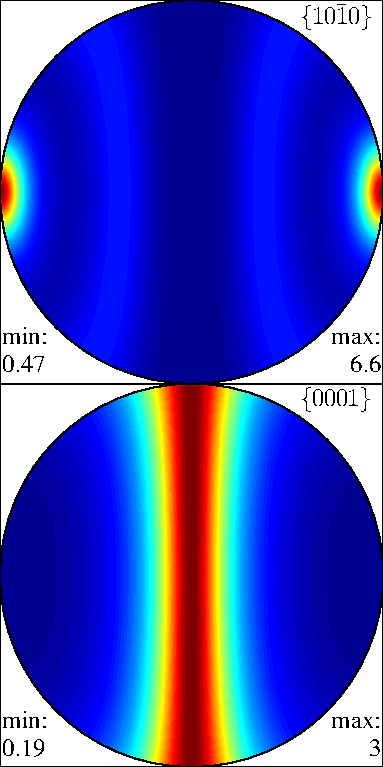
\includegraphics[width=3cm]{pic/fibreodf1}%
      }%
      \only<2>{%
        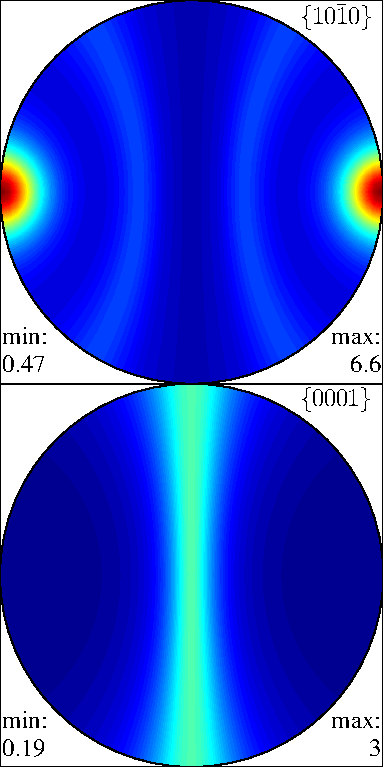
\includegraphics[width=3cm]{pic/fibreodf2}%
      }%
      \only<3|handout:0>{%
        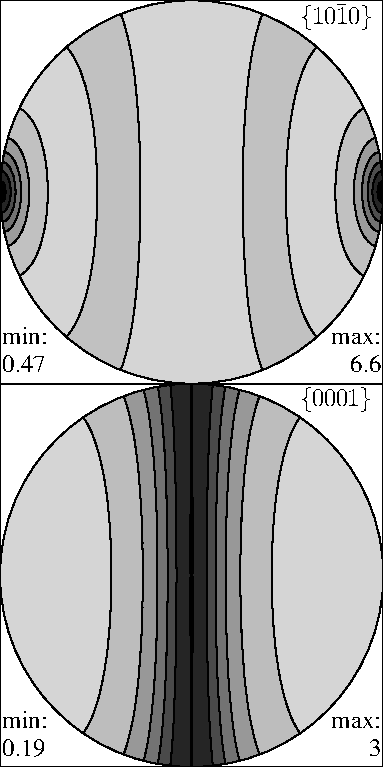
\includegraphics[width=3cm]{pic/fibreodf3}%
      }
    \end{overlayarea}
  \end{column}
  
\end{columns}

  
\end{frame}



\subsection*{Annotations}

\begin{frame}[fragile]
  \frametitle{Add Annotations to Pole Figure Plots}

  
\begin{columns}
  \begin{column}{8.5cm}

\begin{overprint}
  \onslide<1|handout:0>%
  General Syntax:%
\begin{lstlisting}
plot2all(vector,<options>)
\end{lstlisting}
  \onslide<2|handout:1>%
  General Syntax:
\begin{lstlisting}
plot2all(orientation,<options>)
\end{lstlisting}
\end{overprint}

Options:
\begin{lstlisting}
Marker            % marker shape
MarkerSize        % marker size
MarkerFaceColor   % face color
MarkerEdgeColor   % edge color
label             % a label text 
color, background % text colors
\end{lstlisting}

\begin{overprint}
  \onslide<1|handout:0>%
  Example:
\begin{lstlisting}
plot2all([xvector,yvector,zvector],
 'Backgroundcolor','w','Marker','s',
 'MarkerEdgeColor','w','labeled',
 'MarkerFaceColor','k')
\end{lstlisting}
  
  \onslide<2|handout:1>
Example:
\begin{lstlisting}
plot2all(q0,'label','$q_0$',...
   'marker','s','MarkerSize',4,...
   'MarkerFaceColor','r','color','b')
\end{lstlisting}
  
\end{overprint}

\end{column}

  \begin{column}{3.5cm}
    \begin{overlayarea}{3.5cm}{7cm}
      \onslide<1->
      \only<1|handout:0>{%
        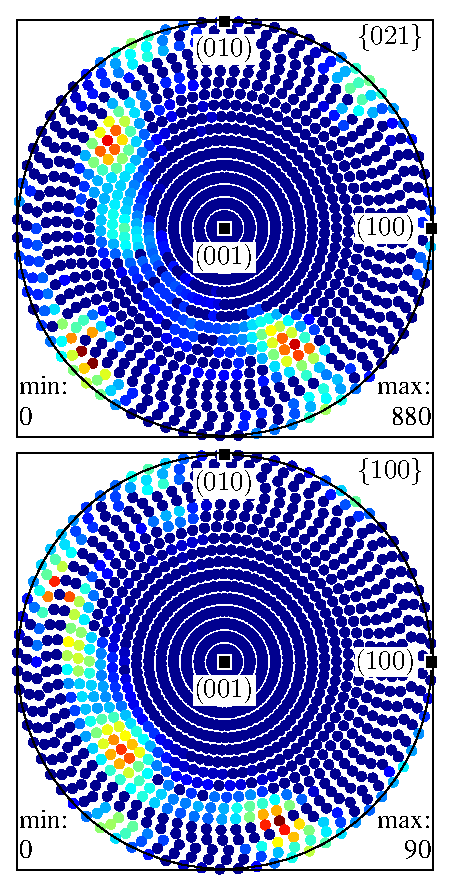
\includegraphics[width=3.5cm]{pic/annotationv}%
      }%
      \only<2>{%
        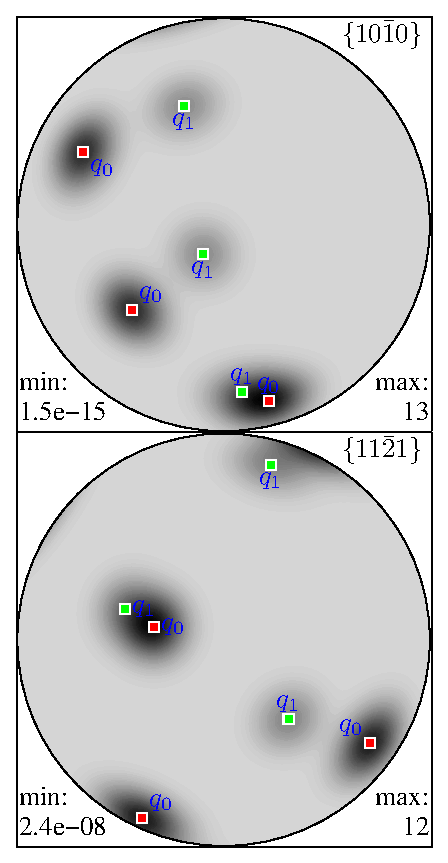
\includegraphics[width=3.5cm]{pic/annotationq}%
      }%
    \end{overlayarea}
  \end{column}

\end{columns}

\end{frame}

\subsection*{Annotations}

\begin{frame}[fragile]
  \frametitle{Add Annotations to ODF Plots}

  
\begin{lstlisting}
plot2all(modalorientation(santafee),'Marker','s',...
  'MarkerSize',6,'MarkerFaceColor','red')
\end{lstlisting}
  
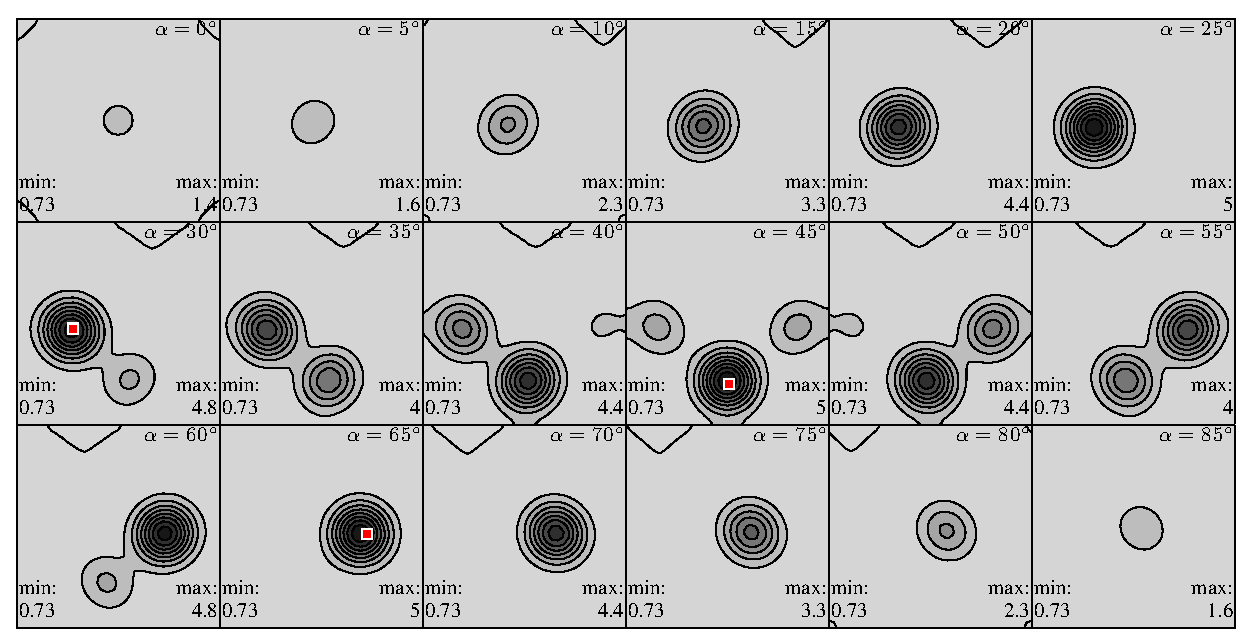
\includegraphics[width=\textwidth]{pic/odfanotate}

\end{frame}

\subsection*{Combined Plots}

\begin{frame}[fragile]
  \frametitle{Combining Different Data Into One Plot}
  
  \begin{columns}
    \begin{column}{8.7cm}
      
      General Syntax:%
\begin{lstlisting}
hold all; hold off
\end{lstlisting}

    Example:
\begin{lstlisting}
plotpdf(odf,h,'contourf','gray')

hold all

plotpdf(ebsd1,h,'MarkerEdgeColor','w',
 'MarkerColor','b','MarkerSize',5)

plotpdf(ebsd2,h,'MarkerEdgeColor','k',
 'MarkerColor','r','MarkerSize',5)

hold off
\end{lstlisting}


    \end{column}
    
    \begin{column}{3.5cm}
      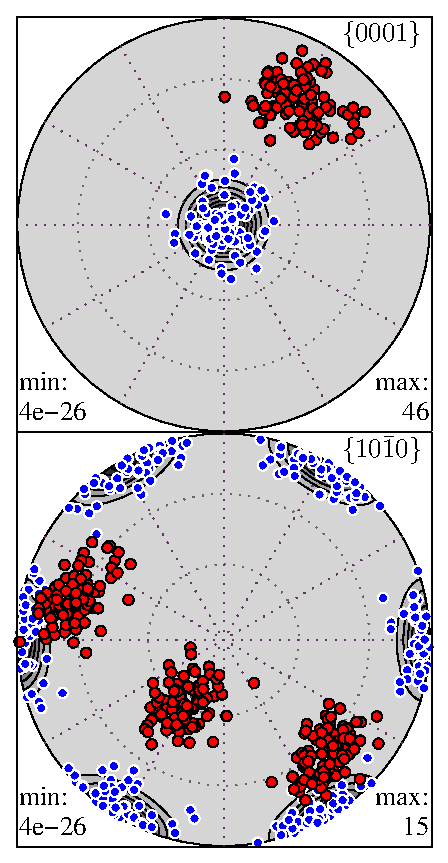
\includegraphics[width=3.5cm]{pic/combined}%
    \end{column}
  \end{columns}

\end{frame}

\subsection*{Export}

\begin{frame}[fragile]
  \frametitle{Exporting Graphics}
    Save a plot:
\begin{lstlisting}
savefigure(filename,<options>)
\end{lstlisting}

    \begin{block}{Formats}
      \begin{itemize}
      \item vector images: pdf, eps, ill 
      \item bitmap images: jpg, tif, png, gif, bmp, pgm, ppm
      \end{itemize}

    \end{block}

    \begin{block}{Options}
\begin{lstlisting}
-append, -tiff, -cmyk, -adobecset
-r<resolution> 
\end{lstlisting}
    \end{block}
\end{frame}

\section{About}

\begin{frame}
%\frametitle{About \MTEX}  

  \author{}
  \date{}
  \institute{}
  \titlegraphic{}  
  \maketitle

  \vskip -2cm

  \begin{block}{Source:}
    \url{http://mtex.googlecode.com}
  \end{block}

  \begin{block}{Contributions by:}
    J. Prestin, D. Potts, J. Keiner, A. Vollrath, F. Bachmann
  \end{block}

  \bigskip

  \centerline{\includegraphics[width=1.5cm]{pic/tu_logo}}




\end{frame}

  
\end{document}








%%% Local Variables: 
%%% mode: latex
%%% TeX-master: .
%%% End: 
